% The dvipsnames option is passed to the xcolor package, which beamer loads
\documentclass[xcolor={dvipsnames}]{beamer}

\usepackage{smpa2152-style}

\title[Sampling]{Sampling}
\author[SMPA 2152]{Data Analysis for Journalism and Political Communication (Fall 2025)}
\date{Prof. Bell}

\begin{document}

%%%%%%%%%%%%%%%%%%%%%%%%%%%%%%%%%%%%%%%%%%%%%%%%%%%%%%%%%%%%%%%%%%
\frame{
\titlepage
}

%%%%%%%%%%%%%%%%%%%%%%%%%%%%%%%%%%%%%%%%%%%%%%%%%%%%%%%%%%%%%%%%%%
\frame{\frametitle{1970 Vietnam War Draft}
\only<1>{
    \centering
    \href{https://www.youtube.com/watch?v=OkJH6sapQMA}{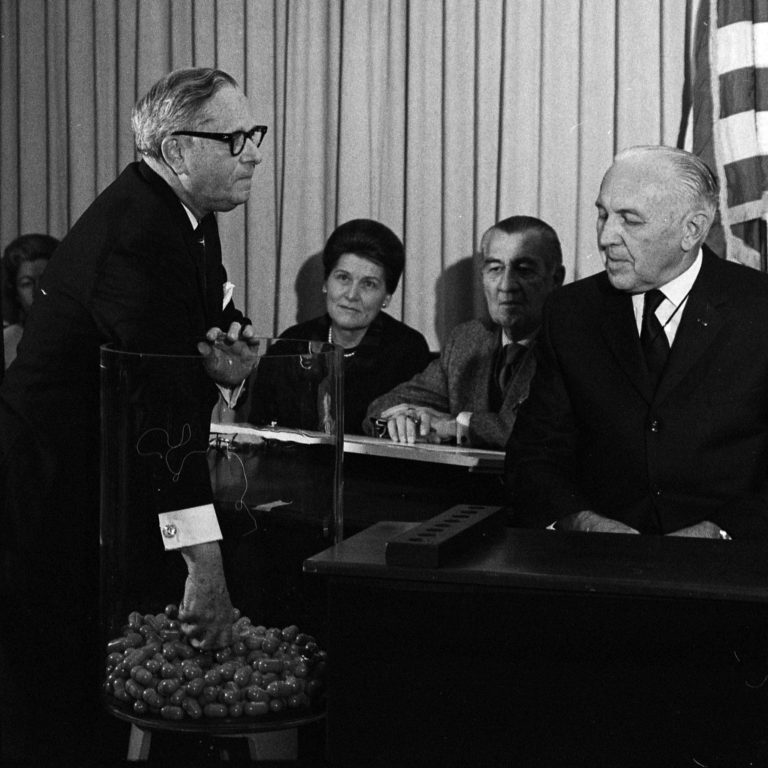
\includegraphics[height = .8\textheight]{lottery_image.jpg}}
}
\only<2>{
    \centering
    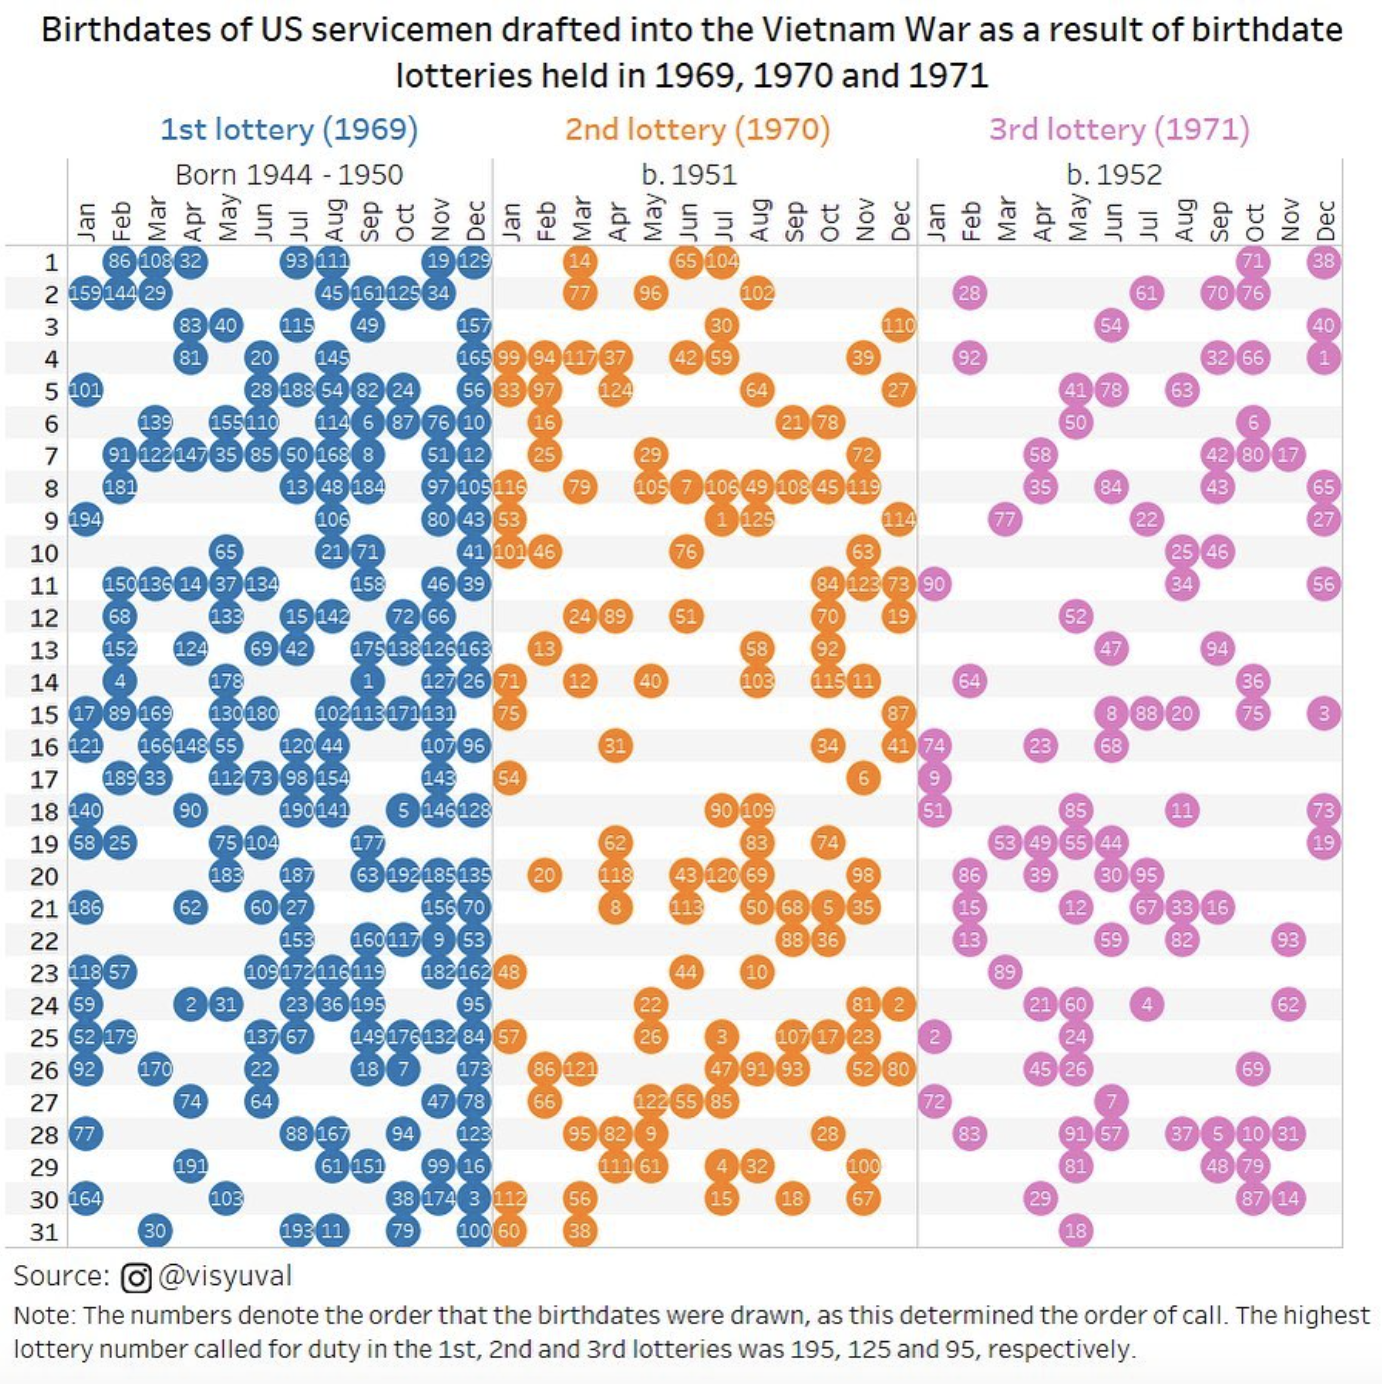
\includegraphics[height = .8\textheight]{vietnam_lottery_data.png}
}
}

%%%%%%%%%%%%%%%%%%%%%%%%%%%%%%%%%%%%%%%%%%%%%%%%%%%%%%%%%%%%%%%%%%
\frame{\frametitle{Definitions}
\begin{itemize}[<+->]
    \item The group we are interested in studying is known as the \textbf{population}
    \item Often, we are not able to count every unit in the population, so we take a \textbf{sample}
    \item Our best guess about the population based on our sample is the \textbf{estimate}
    \item The key to a good estimate is a quality sample, which is determined by two elements:
        \begin{enumerate}
            \item<.-> A \textbf{random sample} of the population
            \item<.-> The \textbf{sample size} is sufficiently large
        \end{enumerate}
\end{itemize}
}

%%%%%%%%%%%%%%%%%%%%%%%%%%%%%%%%%%%%%%%%%%%%%%%%%%%%%%%%%%%%%%%%%%
\frame{
\Large
In-class exercise
}

%%%%%%%%%%%%%%%%%%%%%%%%%%%%%%%%%%%%%%%%%%%%%%%%%%%%%%%%%%%%%%%%%%
\frame{\frametitle{Sample Size}
\begin{itemize}[<+(2)->]
    \item<1-> How many units should you sample from the population? \only<2->{\textbf{It depends on your desired level of certainty.}}
    \item The most common level of certainty is 95\% (the inverse of a \textbf{p-value} of .05, meaning that there is a 5\% chance we are committing Type I error)
    \item In other words, there is a 5\% chance that the true population value is outside of the \textbf{confidence interval}
    \item If we re-sampled the population 100 times, 95 of our estimates would fall within the confidence interval (let's see this in action!)
\end{itemize}
}

%%%%%%%%%%%%%%%%%%%%%%%%%%%%%%%%%%%%%%%%%%%%%%%%%%%%%%%%%%%%%%%%%%
\frame{\frametitle{Margin of Error}
\begin{itemize}[<+->]
    \item The confidence interval for a proportion\footnote{There is a different formula for continuous variables.} is also called the \textbf{margin of error (MOE)}
    \item The 95\% MOE is calculated as:\\
    ~\\
    $1.96 * \sqrt{p * (1 - p) / n}$\\
    ~\\
    where \textit{p} is the proportion and \textit{n} is the sample size
    \item Typically, pollsters will use a proportion (\textit{p}) of .5 to calculate an MOE for the entire poll:\\
    ~\\
    $1.96 * \sqrt{.5 * (1 - .5) / 1000} = .031$\\
    ~\\
    \item We report the estimate with the MOE, e.g., 45 +/- 3.1\%.
\end{itemize}
}

%%%%%%%%%%%%%%%%%%%%%%%%%%%%%%%%%%%%%%%%%%%%%%%%%%%%%%%%%%%%%%%%%%
\frame{\frametitle{Sample Size and the Margin of Error}
\only<1-3,5>{
\begin{itemize}[<+->]
    \item Mathematically, the MOE gets smaller as the sample size increases
    \item Intuitively, the larger our sample size, the less likely we are to draw an ``outlier'' sample and the more likely we are to get a representative sample
    \item But the marginal improvement in the MOE from adding units to the sample decreases as the sample size grows
    \item Remember that the MOE only takes into account the sample size, not the potential for selection bias
\end{itemize}}

\only<4>{
    \centering
    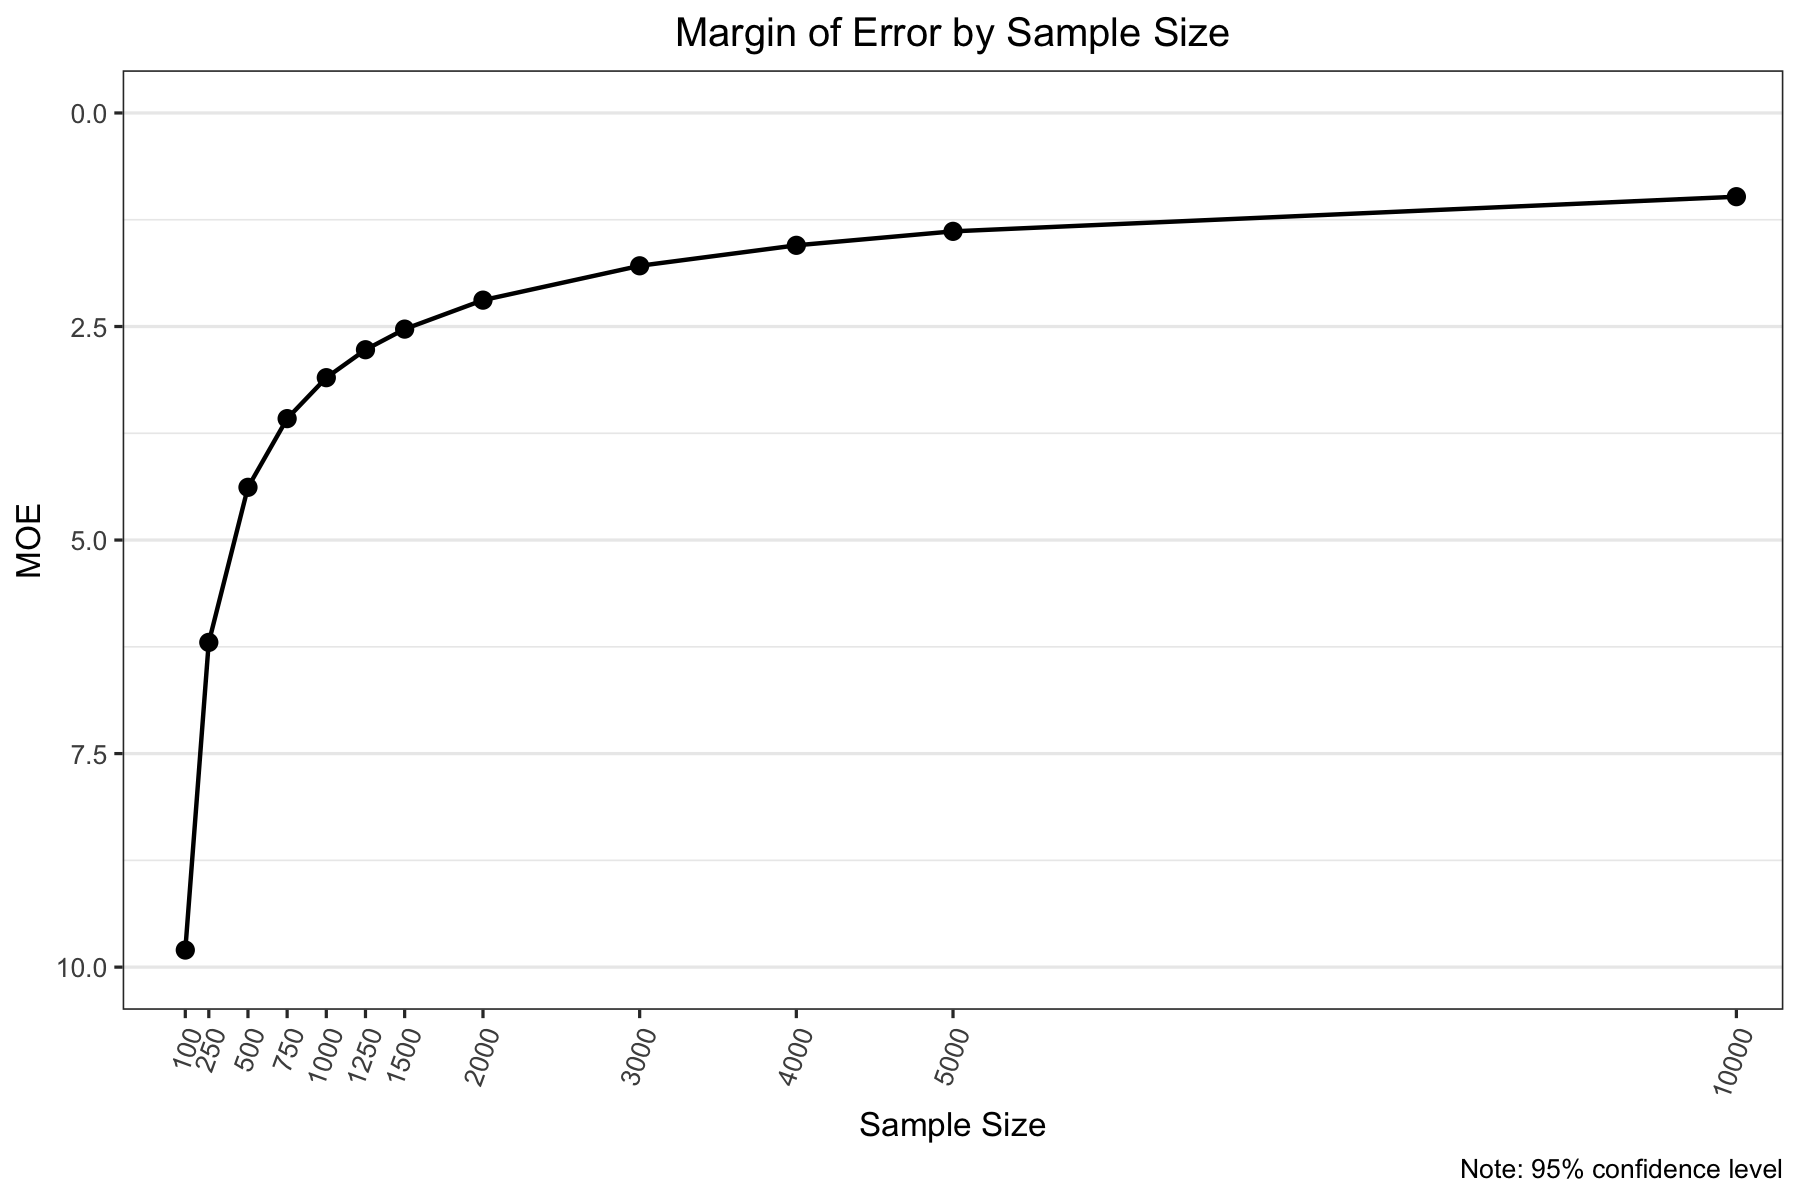
\includegraphics[width=.9\textwidth]{moe_samplesize.png}}
\only<6>{
    \begin{center}
    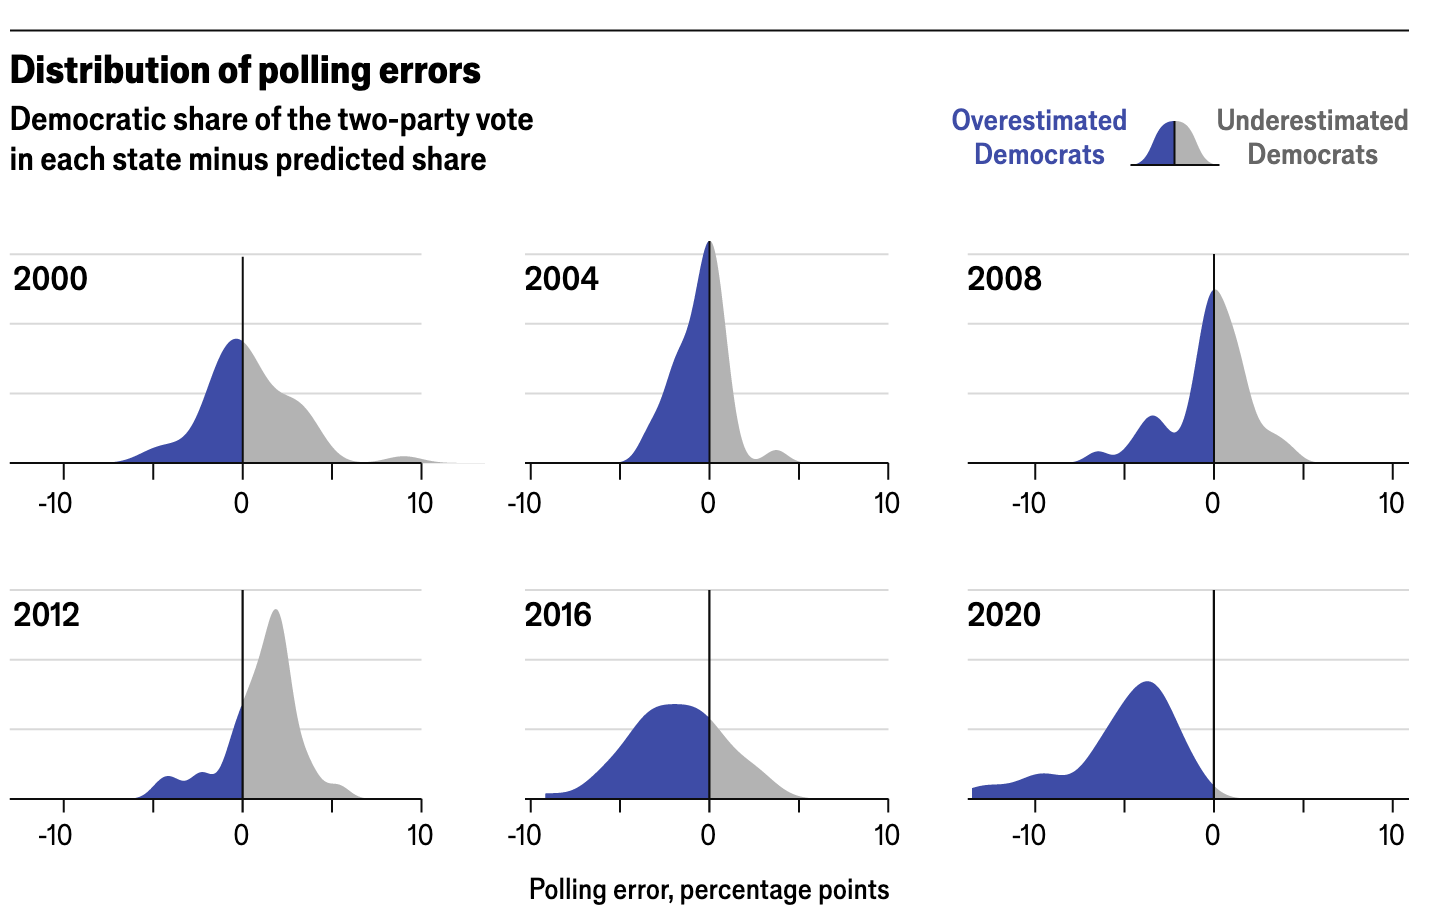
\includegraphics[width=.9\textwidth]{distribution_polling_error.png}
    \end{center}
    {\scriptsize Source: The Economist}
    }
}

\end{document}
